\section{Résultats de l'entraînement}

\subsection{Résultats Théoriques}
Avant même de conclure sur nos résultats expérimentaux, il convient de conclure théoriquement sur la qualité des différentes méthodes implémentées.
En effet, notre solution finale a finalement été d’implémenter la méthode DDPG, mais celle-ci reste critiquable.
En effet, comme nous l’évoquions précédemment il existe plusieurs méthodes permettant de mettre en place des espaces d’actions continues pour un agent.
Globalement, nous avons eu le choix entre deux méthodes : 
Le DDPG dont nous avons rapidement expliqué le fonctionnement et l’estimation de loi normale.
Cette méthode est assez intuitive d’autant qu’elle fonctionne de façon similaire aux méthodes plus conventionnelles.
L’objectif de cette méthode est de faire estimer à un agent autant de gaussienne qu’il y a de sorties.
On choisit ensuite l’action en fonction de la gaussienne que ressort le réseau de neurones.
Le réseau nous ressort donc 2 paramètres (mu,sigma) : l'espérance et l'écart-type de la loi normale.
\begin{figure}[H]
    \centering
    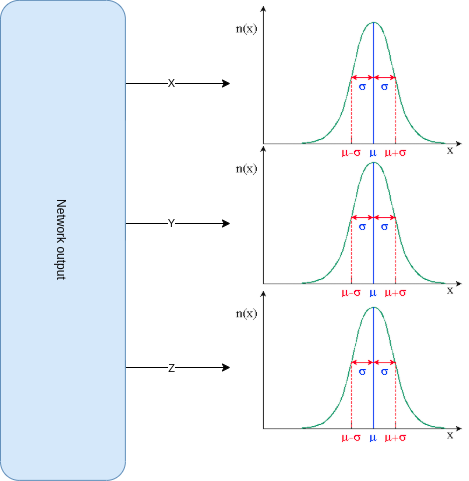
\includegraphics[width=0.5\textwidth]{./image_RL/image37.png}
    \caption{  estimation loi normal  }
\end{figure}
Cette méthode nous permet donc d’estimer une policy stochastique plutôt que le DDPG qui estime une policy déterministe. 
Les avantages de cette méthode sont multiples.
La première et plus importante, est le fait qu’avec une telle estimation on peut critiquer nous même l’action que prend un réseau.
En effet, on entend souvent dire dans le monde de l’industrie que les réseaux de neurones sont des boîtes noires pour lesquelles aucune interprétation n’est possible.
Avec la méthode DDPG on ressort trois actions qu’on ne peut pas du tout critiquer. 
Or avec cette méthode, le réseau ressort une espérance que l’on peut voir comme l’action que le réseau veut prendre et l’écart-type que l’on peut voir comme la confiance qu’accorde le réseau à l’action qu’il propose. On peut donc critiquer les actions que prend le réseau et agir en fonction. On aura plus de confiance à laisser un réseau prendre une action pour laquelle il est sûr à 80% qu’une action pour laquelle il n’est sûr qu’à 10 %.
Aussi le problème du DDPG est que nous devons nous même réaliser la phase d’exploration en introduisant une partie aléatoire.
En effet, pour apprendre au robot des nouvelles actions qui pourraient être meilleures que celles qu’il prend déjà, il faut ajouter une partie aléatoire aux actions qu’il prend dans la phase d’entraînement.
Pour la méthode de DDPG on se sert généralement d’un bruit gaussien qu’on ajoute aux sortie. Ce bruit étant totalement disjoint de l’agent, il n’évolue pas en fonction de son apprentissage. Ainsi, il faut que l’opérateur (nous) règle la loi normale en fonction de la phase d’apprentissage dans laquelle se trouve l’agent.
Ce qui n’est pas le cas pour la méthode d’estimation gaussienne.
En effet, on va choisir l’action directement en lien avec la loi normale estimée par l’agent.
Plus l’agent va apprendre, plus il va estimer une loi réduite, plus la phase d’exploration sera adaptée à son apprentissage.

\subsection{Résultats expérimentaux}
Dans la précédente partie nous avons parlé de la méthode d’estimation des lois gaussiennes. Cette méthode semble être plus qu’optimale pour les méthodes de renforcement pour champ d’actions continu.
Malheureusement, en pratique cette méthode marche moins bien que la méthode déterministe.
Le problème est lié au fait que les sorties estimées par l’agent sont contraintes physiquement. En effet, nous ne pouvons envoyer au drone qu’un champ d’actions réduit. Or la loi normale est définie sur tout R.

\begin{figure}[H]
    \centering
    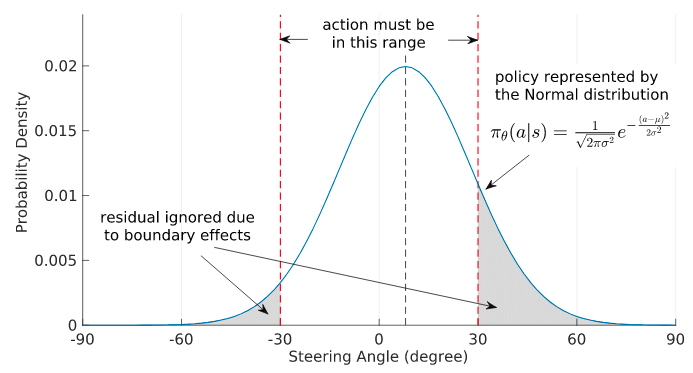
\includegraphics[width=0.5\textwidth]{./image_RL/image14.png}
    \caption{  limites du système   }
\end{figure}

Ainsi bien que l’approche stochastique soit plus optimisée théoriquement, elle fonctionne moins en pratique.

Nous avons donc décidé de mettre en place la méthode ddpg pour laquelle nous allons vous présenter nos résultats.

\subsection{ANN simple}

\begin{figure}[H]
    \centering
    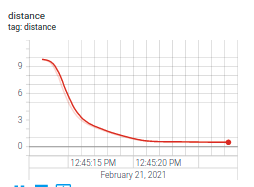
\includegraphics[width=0.5\textwidth]{./image_RL/image36.png}
    \caption{  réponse à une consigne en échelon   }
\end{figure}

Comme vous pouvez le voir sur notre réseau ANN, notre agent part avec une distance d’environ 10 mètres de sa cible. 
Il met environ 5 secondes pour atteindre celle-ci. En revanche, on voit qu’il conserve un certain biais de l’ordre de 50 cm. Les possibilités sont multiples.
D’une part, le réseau peut être optimisé et entraîné plus longtemps. Pour ces résultats, le réseau a été entraîné seulement 1 heure.
Aussi, Gazebo génère son propre bruit capteur. Donc le robot peut avoir du mal à atteindre la cible au même titre que d’autres méthodes plus conventionnelles dû à ce bruit.
En effet, le réseau prend en entrée les données capteurs bruitées.
Il faudrait peut-être utiliser un kalman pour estimer la distance du robot et avoir de meilleurs résultats.

\subsection{LSTM}

\begin{figure}[H]
    \centering
    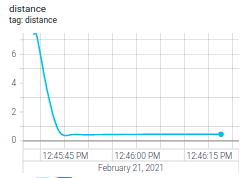
\includegraphics[width=0.5\textwidth]{./image_RL/image16.png}
    \caption{ réponse à une consigne en échelon pour le LSTM    }
\end{figure}

On remarque que le réseau LSTM est un peu plus rapide que le réseau ANN simple. En revanche, comme celui-ci le biais demeure.

\subsection{Convolution}
La méthode d’asservissement par réseau à convolution n’a pas donné de résultats concluants. En effet, l’objectif du drone était de se poser sur une plateforme mobile en utilisant uniquement le retour image.
Or le robot ne peut pas estimer la vitesse de la plateforme avec ce retour image.
La solution aurait été de mettre une couche LSTM en sortie du CNN.
Malheureusement nous étions limités par le temps.

